% -*- coding: utf-8 -*-

\cleardoublepage
\plainifnotempty

\chapter{データベースシステムの夜明け}

\begin{flushright}
はやみず
\end{flushright}

\lettrine{デ}ータベースシステム無しでは、今日の社会は成り立たないと言って
良いでしょう。社会が高度に情報化された現在、世界中で大量のデジタルデータ
が日々生み出され、飛び交い、消費され、そして蓄積されてゆきます。2011年に
人類の生み出したデータ量は1,800ペタバイトにのぼります。一方で、膨大なデジ
タルデータは、単に生み出され、蓄積されてゆくだけではただのゴミも同様です。
必要なときに必要なデータが取り出せるよう、適切に管理してゆかなければなり
ません。そのための根幹たる存在が、データベースシステムなのです。

みなさんが馴染みのあるであろう MySQL や PostgreSQL、あるいは Oracle といっ
たデータベースシステムは、正確には「リレーショナルデータベースシステム」
と呼ばれています。リレーショナルデータベースシステムの歴史を辿ると、その
起源はある一篇の論文に遡ることができます。

その論文こそが、Edgar F.  Coddにより1970年に発表された ``A Relational
Model of Data for Large Shared Data Banks'' です。この論文は、リレーショ
ナルデータベースの最も重要な基礎となる{\bf リレーショナルデータモデル}を
提唱したもので、いわばデータベースシステム分野における金字塔です。古典力
学を Newton が拓き、相対性理論を Einstein が拓いたとするならば、データベー
スにおける一大分野であるリレーショナルデータベースを拓いたのは間違いなく
Edgar Codd その人といって間違いないでしょう。

そして、Codd によりリレーショナルモデル提唱から数年の後に、UNIXで動作する
世界初のリレーショナルデータベースシステムの開発プロジェクトが立ち上がり
ます。Michael Stonebraker率いる{\bf INGRESプロジェクト}です。Coddにより確
立されたリレーショナルデータベースシステムの基礎理論を、実際に動くソフト
ウェアとして実現し、そしてそれを世に広めたのがINGRESなのです。

本稿では、Coddによるリレーショナルデータモデルの提唱から、INGRESプロジェ
クトの黎明期の記録を辿り、現代の社会を支えるデータベースシステムがいかに
して創り上げられたのか、その歴史を紐解いてみようと思います。

{\small ※ これ以降、特に断りのない場合、リレーショナルデータベースシステムを指して
単にデータベースシステムと書くことがあります。}

\section{時代はリレーショナルへ}

1960年代以前のデータベースシステムは階層型データモデル、やネットワーク型
データモデルというデータモデルに基づいて構築されていました。

\begin{figure}[tb]
 \begin{minipage}{0.48\textwidth}
  \begin{center}
   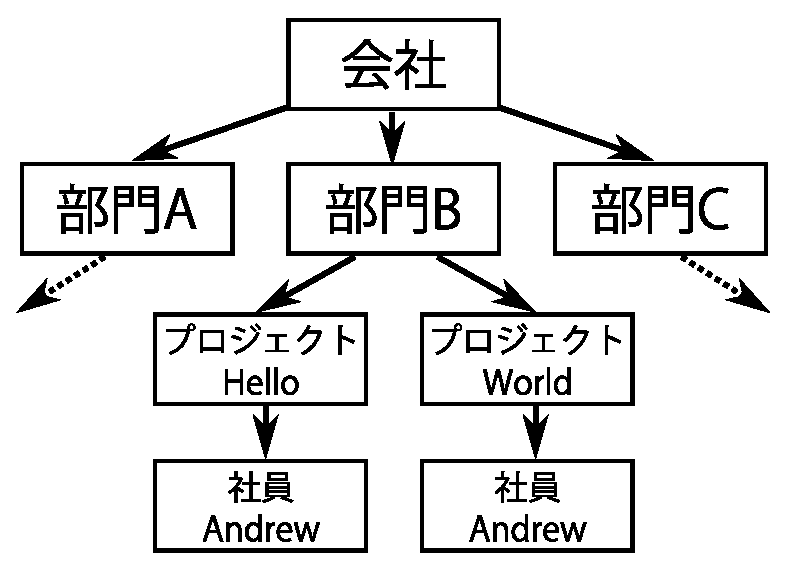
\includegraphics[width=5cm]{hayamiz/images/hierarchical-data-model.eps}
   \caption{階層型データモデル}
   \label{214539_12Jul12}
  \end{center}
 \end{minipage}
 \begin{minipage}{0.48\textwidth}
  \begin{center}
   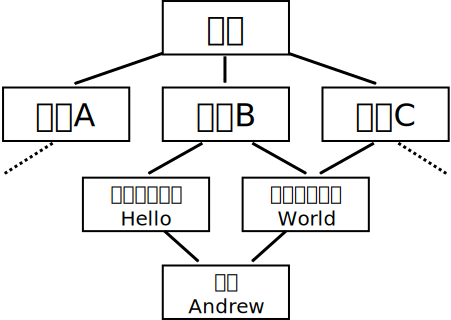
\includegraphics[width=5cm]{hayamiz/images/network-data-model.eps}
   \caption{ネットワーク型データモデル}
   \label{214707_12Jul12}
  \end{center}
 \end{minipage}
\end{figure}

階層型データモデルというのは、木構造を用いてデータを組織化したデータモデ
ルです。たとえば会社組織を階層型データモデルで表そうと思うと、会社の下に
は複数の部門が属しており、各部門の下には複数のプロジェクトがあり、各プロ
ジェクトの下には社員が属している、というようにスキーマを定義してゆきます
(図\ref{214539_12Jul12})。ここで、例えば2つのプロジェクトHelloとWorldに属
する1人の社員Andrewがいたとしたらどうでしょう。階層型データモデルでは、あ
るデータの実体(ここでは1人の社員)は親となるデータの実体(プロジェクト)
を複数持つことができません。そのため、各プロジェクトごとにAndrewのデータ
を持つことになり、データの重複が生じてしまいます。また、部門Bと部門Cが共
同でプロジェクトWorldを運営していることを表現しようと思うと、プロジェクト
のデータに加えてその下にぶら下がっている社員のデータも併せてコピーしなけ
ればなりません。このような欠点を克服したのがネットワーク型データモデルで
す(図\ref{214707_12Jul12})。ネットワーク型データモデルでは、データの実
体が複数の親を持つことができる有向グラフをデータ構造として採用したため、
前述のようなデータ重複の問題は発生しません。

ネットワーク型モデルによりより一般的なデータ構造を表現できるようにはなり
ました。しかし、階層型モデルやネットワーク型モデルに基づくデータベースは、
データのアクセスに一つ大きな問題を抱えていました。これらのデータベースに
おいてデータの問い合わせを行う際には、データの構造がどのようになっている
かを把握し、そしてどのような手順でデータを取得するかを利用者が知っている
必要があったのです。例えば図\ref{214707_12Jul12}のデータベースにおいて社
員Andrewのデータを取得するためには、「会社のデータを読みとり、部門Bのデー
タを読み取り、プロジェクトHelloのデータを読み取り、社員Andrewのデータを読
み取る」という手順を指定してあげなければなりません。このように、欲しいデー
タにアクセスするための``how'' をもって問い合わせを行うデータベースシステ
ムは、ユーザがデータの案内(navigation)をするという意味で{\bf ナビゲーショ
ナルデータベースシステム}と呼ばれます。

もしもナビゲーショナルデータベースシステムにおいて、図
\ref{214707_12Jul12}の会社で組織改変があり、各部門の下には課が設置され、
その下にプロジェクトが属するという構造にデータベースが修正されたとしたら
どうなるでしょう。これまで社員のデータにアクセスするアプリケーションは会
社→部門→プロジェクト→社員とたどっていましたが、会社→部門→課→プロジェ
クト→社員とたどるように修正しなければなりません。このように、ナビゲーショ
ナルデータベースシステムでは、ある特定のデータのみに興味があったとしても、
その上位構造に変化があった時にはデータにアクセスする方法を再構成しなけれ
ばなりませんでした。

歴史的には、階層型モデルはそのシンプルさ故に初期のデータベースシステムに
おいて採用され、その後により一般的なデータの組織化を行うことができるよう、
ネットワーク型モデルが発明されます。1969年にはCODASYLという委員会によって、
ネットワーク型データモデルの標準化が行われ、データベースシステムの情勢は
階層型モデルからネットワーク型モデルに移るかと思われました。

そこに登場したのが、1970年\footnote{正確にはリレーショナルデータモデルの
論文は1969年にIBMの社内技術報に掲載され、翌1970年に米国コンピュータ学会の
論文誌に掲載されます。}にCoddによって提唱されたリレーショナルデータモデル
です。リレーショナルデータモデルは、数学の集合論に基づいてデータを組織化
する方法論であり、階層型モデルやネットワーク型モデルのようにデータアクセ
スのための具体的なアルゴリズムを内包しません。ユーザは「どんなデータが欲
しいか」を記述するたけで、具体的なアクセス方法はデータベース側が判断して
データを取得することができます。つまり、ナビゲーショナルデータベースシス
テムでは ``how'' を与えなければデータのアクセスが行えなかったのですが、リ
レーショナルデータベースは ``what'' を与えるだけでデータのアクセスが可能
となります\footnote{リレーショナルモデルの数学的な定義や、なぜそれにより
``what''でデータの問い合わせが可能となるのかの説明については、それだけで
一冊の本になってしまうので他書に譲ります。}。

また階層型モデルなどとは異なり、リレーショナルモデルはしっかりとした数学
的基礎の上に成り立っており、後のデータベースシステム研究の大きな基盤とな
りました。これまでプログラマによるある種の職人芸の上に成り立っていたデー
タベースシステムは、リレーショナルデータモデルの登場によって科学の領域へ
と押し上げられたのです。

ちなみに、データベースのお勉強をした人たちは、ドメイン、リレーション、タ
プル、主キー、外部キー、○○正規形という言葉に聞き覚えがあるかもしれませ
んが、これら教科書に載っているリレーショナルデータモデルのかなりの部分が
1970年の論文の段階で体系的にまとめられています。もちろん現在のリレーショ
ナルデータモデルは様々な改良が加えられていますが、その基本的な骨子はほぼ
そのままの形で残っています。この論文はタイトルで検索すればオンラインで読
むことができます。自分の勉強した知識と照らし合わせながら読んでみると面白
いのではないでしょうか。

\section{INGRESプロジェクト始動}

リレーショナルデータモデルがCoddによって提唱されてから3年後、その論文が一
人の若き研究者の目に留まりました。その人こそ、INGRESプロジェクト、そして
後のデータベース業界全体を率いる存在となる Michael Stonebraker です。
1971年にミシガン大学で博士号を取得し、UC Berkeleyで研究職についたばかりの
Stonebraker はテニュアトラック\footnote{テニュアとは大学における終身雇用
資格のことです。若手研究者は任期の限られた研究職につき、テニュア獲得を目
指して研究業績を積み上げてゆく、というの米国における一般的な研究者のキャ
リアパスです。このテニュア獲得のための若手研究者が通る道をテニュアトラッ
クと呼びます。テニュアトラックでいかに論文を``量産''できる研究ネタを選ぶ
かというのは、若手研究者にとっては人生に関わる重要な決断なのです。}を走り
始めたばかりであり、何か良い研究のネタはないかと思案していたところでした。
そんな Stonebraker にとって、リレーショナルモデルは恰好の研究対象だったの
でしょう\footnote{ちなみに Stonebraker の博士論文は ``The Reduction of
Large Scale Markov Models for Random Chains'' というタイトルで、もともと
は数学寄りの研究をしていたようです。 }。リレーショナルデータモデルに出会っ
た Stonebraker は、Eugene Wong と共にリレーショナルデータベースシステムの
実装に乗り出します。こうしてINGRESプロジェクトは始まりました。

% http://genealogy.math.ndsu.nodak.edu/id.php?id=31091

INGRESという名前は、{\bf IN}teractive {\bf G}raphic and {\bf RE}trieval
{\bf S}ystem の頭文字をとったもので、本来は UC Berkeley の経済学の研究チー
ムのために、地理情報をグラフィカルに表示するためのシステム研究として予算
を獲得していたプロジェクトでした。そこは本音と建前で、まずはデータを効率
的に取得するためのデータベースシステムが必要だ、ということで Stonebraker
達はデータベースシステムの開発にのめりこんでゆきます。



System R disる

\section{INGRESのtechnical detail}

Design and Implementation of INGRES

Retrospective on Database Systems あたりをベースに書く

\section{Ingres Corporation設立}

後に Relational Technology Inc.,

Oracleとの絡みはどうする?

\section{POSTGRESプロジェクト}

Post-INGRES

\section*{参考文献}

\begin{itemize}
 \item E. F. Codd, ``A Relational Model of Data for Large Shared Data
       Banks'', {\it Communications of the ACM}, Volume 13, Number 6,
       1970
 \item M. Stonebraker, G. Held, E. Wong, P. Kreps, ``The design and
       implementation of INGRES'', {\it ACM Transactions on Database
       Systems},
Volume 1, Issue 3, 1976
 \item M. Stonebraker, ``Retrospection on a database system'', {\it ACM
       Transactions on Database Systems}, Volume 5, Issue 2, 1980
 \item National Research Council, ``Funding a Revolution: Government
       Support for Computing Research'', Natl Academy Pr, 1999
\end{itemize}